%% on the state space {0,1,2,3,...}. This is the same continuous time Markov chain as in a birth–death process. The state space diagram for this chain is as below.
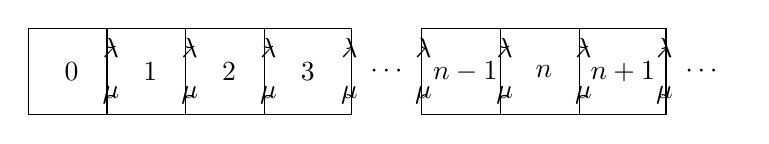
\begin{tikzpicture}%[->,>=stealth',shorten >=1pt,auto,node distance=2cm,semithick]
  % \tikzstyle{every state}=[fill=white,draw=black,text=black,minimum size=1.1cm]
  \tikzstyle{state}=[fill=white,draw=black,text=black,minimum size=1.1cm]
 
  \node[state] (A) {0};
  \node[state] (B) [right of=A] {$1$};
  \node[state] (C) [right of=B] {$2$};
  \node[state] (D) [right of=C] {$3$};
  \node[minimum size=1cm] (E) [right of=D] {$\cdots$};
  \node[state] (F) [right of=E] {$n-1$};
  \node[state] (G) [right of=F] {$n$};
  \node[state] (H) [right of=G] {$n+1$};
  \node[minimum size=1cm] (I) [right of=H] {$\cdots$};
 
  \path (A) edge [bend left] node {$\lambda$} (B);
  \path (B) edge [bend left] node {$\mu$} (A);
  \path (B) edge [bend left] node {$\lambda$} (C);
  \path (C) edge [bend left] node {$\mu$} (B);
  \path (C) edge [bend left] node {$\lambda$} (D);
  \path (D) edge [bend left] node {$\mu$} (C);
  \path (D) edge [bend left] node {$\lambda$} (E);
  \path (E) edge [bend left] node {$\mu$} (D);
  \path (E) edge [bend left] node {$\lambda$} (F);
  \path (F) edge [bend left] node {$\mu$} (E);
  \path (F) edge [bend left] node {$\lambda$} (G);
  \path (G) edge [bend left] node {$\mu$} (F);
  \path (G) edge [bend left] node {$\lambda$} (H);
  \path (H) edge [bend left] node {$\mu$} (G);
  \path (H) edge [bend left] node {$\lambda$} (I);
  \path (I) edge [bend left] node {$\mu$} (H);
\end{tikzpicture}
